\documentclass{homework}
\course{Math 6802}
\author{Jim Fowler}
\input{preamble}

\usepackage{tikz}
\usetikzlibrary{arrows,chains,matrix,positioning,scopes}

\makeatletter
\tikzset{join/.code=\tikzset{after node path={%
\ifx\tikzchainprevious\pgfutil@empty\else(\tikzchainprevious)%
edge[every join]#1(\tikzchaincurrent)\fi}}}
\makeatother

\tikzset{>=stealth',every on chain/.append style={join},
         every join/.style={->}}

\begin{document}
\maketitle

\begin{inspiration}
``The notions category and functor were not formulated or put in print until the idea of a natural transformation was also at hand.''
\byline{Saunders Mac Lane}
\end{inspiration}

\section{Terminology}

\begin{problem}
  What is a flat $R$-module?
\end{problem}

\begin{problem} For chain complexes $C_\star$ and $D_\star$, describe
$C_\star \otimes D_\star$ as a chain complex.
\end{problem}

\begin{problem} For chain complexes $C_\star$ and $D_\star$, describe
$\Hom(C_\star,D_\star)$ as a chain complex.
\end{problem}

\section{Numericals}

\begin{problem}
  Compute $\Tor(\Z/m,\Z/n)$.
\end{problem}

\begin{problem}
  Compute $\Ext(\Z/m,\Z/n)$.
\end{problem}

\section{Exploration}

\begin{problem}
  An extension of $A$ by $B$ is a short exact sequence
  $$
  0 \to A \to E \to B \to 0.
  $$
  Two extensions $0 \to A \to E \to B \to 0$ and $0 \to A \to E' \to B
  \to 0$ are said to be \textit{equivalent} if there is a map $f : E \to E'$ so
  that the following diagram
  \begin{center}
  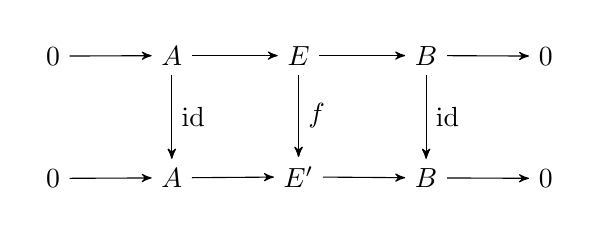
\begin{tikzpicture}
  \matrix (m) [matrix of math nodes, row sep=3em,
    column sep=3em]
    { 0 & A  & E  & B  & 0 \\
      0 & A & E' & B & 0 \\ };
  { [start chain] \chainin (m-1-1);
    \chainin (m-1-2);
    { [start branch=A] \chainin (m-2-2)
        [join={node[right] {$\mathrm{id}$}}];}
    \chainin (m-1-3);
    { [start branch=B] \chainin (m-2-3)
        [join={node[right] {$f$}}];}
    \chainin (m-1-4);
    { [start branch=C] \chainin (m-2-4)
        [join={node[right] {$\mathrm{id}$}}];}
    \chainin (m-1-5); }
  { [start chain] \chainin (m-2-1);
    \chainin (m-2-2);
    \chainin (m-2-3);
    \chainin (m-2-4);
    \chainin (m-2-5); 
}
\end{tikzpicture}
\end{center}
commutes.  Show that the set of equivalence classes of extensions of
$A$ by $B$ is naturally isomorphic to $\Ext(B,A)$.
\end{problem}

\begin{problem}
Let's add this abstract machinery to our toolbox.
  Often after much work, we find a short exact sequence
  \(
   0 \to A \to B \to C \to 0
  \) of abelian groups $A$, $B$, $C$, and we have an explicit
description of $A$ and $C$, but we seek an explicit description of
$B$.  When is this easy to do?  When is it hard?
\end{problem}

\begin{problem}
  For chain complexes $C_\star$ and $D_\star$,
  explain why a chain map $f : C_\star \to D_\star$ is a $0$-cycle in the chain complex
  $\Hom(C_\star,D_\star)$.

 What is a chain homotopy $f \simeq g$ in terms of the chain complex 
 $\Hom(C_\star,D_\star)$?
\end{problem}

\section{Prove or Disprove and Salvage if Possible (PODASIP)}

\begin{problem}
  For an abelian group $G$, the maps $H \mapsto \Ext(H,G)$ and $H \mapsto \Ext(G,H)$ are functors.
\end{problem}

% \begin{problem} Suppose $0 \to A \to B \to C \to 0$ is an exact
% sequence of abelian groups.  Then for an abelian group $G$, the
% sequence
%   \[
%     0 \to \Hom(G,A) \to \Hom(G,B) \to \Hom(G,C) \to 0
%   \]
%   is exact.
% \end{problem}

\end{document}
